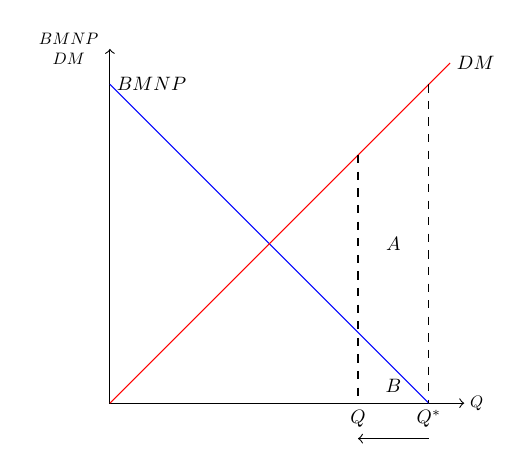
\begin{tikzpicture}[scale=0.9]
	% Ejes
		\draw[<->] (0,5)  node [text width=15mm,text centered, scale=0.6, left] {$BMNP$ $DM$}-- (0,0) -- (5,0) node [scale=0.6, right] {$Q$};
	
	% Rectas
		\draw[blue] (0,4.5) node [right, scale=0.7, black] {$BMNP$} -- (4.5,0) node [below, scale=0.7, black] {$Q^\ast$};
		\draw[red] (0,0) -- (4.8,4.8) node [right, scale=0.7, black] {$DM$};
	
	% Rectas sombreadas
		\draw[dashed] (4.5,4.5) -- (4.5,0);
		\draw[dashed] (3.5,3.5) -- (3.5,0)  node [below, scale=0.7, black] {$Q$};
	
	% A y B
		\draw (4,2.25) node [scale=0.7, black] {$A$};
		\draw (4,0.25) node [scale=0.7, black] {$B$};
	
	% Flechas
		\draw[->] (4.5,-0.5) -- (3.5,-0.5);
\end{tikzpicture}